\documentclass[12pt,twoside,a4paper]{report}

\usepackage{amsfonts,amssymb,amsmath,epsfig}
\usepackage[portuguese,brazil]{babel}    % dá suporte para os termos na língua portuguesa do Brasil
%\usepackage[latin1]{inputenc} % dá suporte para caracteres especiais como acentos e cedilha
%\usepackage{ucs}
\usepackage[utf8]{inputenc}
\usepackage[T1]{fontenc}      % Lê a codificação de fonte T1 (font encoding default é 0T1).
\usepackage{ae}               % Fonte "Almost European"
%% \usepackage[portuguese]{babel}
%% %\usepackage[brazil,english]{babel}
%% %\usepackage[english,brazil]{babel}
%% \usepackage[T1]{fontenc}
\usepackage{indentfirst}
\usepackage{graphicx}

% ,fleqn] - Alinha as equações a esquerda ao invés de centraliza-las
%\setlength{\mathindent}{1cm} % determina o espaçamento entre a margem
                              % esquerda e as equações
                              
\usepackage{fancyhdr}
\usepackage[T1]{fontenc}
\usepackage{ae}
\usepackage{color}
\usepackage[printonlyused]{acronym}
%\usepackage{float} %put images where they are declared
%\floatplacement{figure}{H}
\usepackage{amsmath}
\usepackage{amsfonts}
\usepackage{hyperref}
%---- Tamanho das Paginas ----

%\oddsidemargin  =   2 mm
%\evensidemargin = -12 mm
\oddsidemargin  =  1 mm  %-5
\evensidemargin =  1 mm %-5
\textwidth      = 170 mm %170
\textheight     = 215 mm %235
\topmargin      = 8 mm %-10
\topskip        =  10  mm %10
\headsep        =  6 mm %10
\footskip       =   0 mm

%---- Espaçamento entre as linhas ----

\newcommand{\blst}{1.5} %{1.15}
\renewcommand{\baselinestretch}{\blst}

%---- Formato das Paginas ----

\pagestyle{headings}
\raggedbottom                 %  impede o ajustamento vertical

%---- Especificacoes sobre figuras ----

\setcounter  {topnumber}      {2}
\setcounter  {bottomnumber}   {2}
\setcounter  {totalnumber}    {2}
\renewcommand{\topfraction}   {1}
\renewcommand{\bottomfraction}{1}
\renewcommand{\textfraction}  {0}

%---- Formatando os títulos ----

\usepackage[bf,rm,compact]{titlesec}
\font\bigrm = cmr10 at 40pt
\titleformat{\chapter}[display]
            {\normalfont\huge\sffamily}
%            {\thispagestyle{empty}\normalfont\huge\sffamily}
            {\rightline{\normalfont\bigrm{\thechapter}}}
            {-2cm}
            {\bfseries}
            [{\vspace{-5mm}\hrulefill\\[.8ex]}]
\titlespacing{\chapter}
            {0cm}{0.5cm}{1.5cm}

%---- Headers ----

\usepackage{fancyhdr}
\pagestyle{fancyplain}
\renewcommand{\chaptermark}[1]{\markboth{\thechapter.\ #1}{} }
\renewcommand{\sectionmark}[1]{\markright{\thesection\ #1}}
\lhead[\fancyplain{}{\bfseries\thepage}]
       {\fancyplain{}{\small\slshape\bfseries\leftmark}}
\rhead[\fancyplain{}{\small\slshape\bfseries\rightmark}]
       {\fancyplain{}{\bfseries\thepage}}
\cfoot[\fancyplain{\bfseries\thepage}{}]
       {\fancyplain{\bfseries\thepage}{}}
\renewcommand{\headrulewidth}{0.3pt}

%---- Especificacoes Numeração ----

\setcounter{secnumdepth}{1}   %  numera apenas ate as seções
\setcounter{tocdepth}{1}      %  inclui no índice somente as seções

%%\input{hifen.tex}



\begin{document}

%%%%%%%%%%%%%%%%%%%%%%%%%%%%%%%%%
\pagestyle{plain}
%\pagenumbering{arabic}
\pagenumbering{roman}
\thispagestyle{empty}
\begin{center}

{\Large \sc
Universidade Estadual de Campinas \\
Instituto de Física {\em Gleb Wataghin} \\
\vspace{0.5cm}
F 896 - Monografia}

\vspace{2cm}

{\huge Estudo sobre

\bigskip

números mágicos dos \textit{clusters} de prata}

\vspace{2.5cm}

\end{center}

\begin{center}

{\large Maria Helena Gonçalves} \\
E-mail: mariahelenags10@gmail.com

\vspace{2.7cm}

%\noindent {\Large{Orientador:} Prof. Dr. Pedro Orientador} \\


%\vspace{1cm}


%\begin{tabular}{l}
{Orientador: Prof. Dr. Varlei Rodrigues}\\
E-mail: varlei@ifi.unicamp.br \\
Departamento de Física Aplicada \\
Instituto de Física {\em Gleb Wataghin}\\
Universidade Estadual de Campinas
%\end{tabular}

\end{center}

\vspace{0.5cm}

\begin{center}

\noindent {\Large{Campinas-SP}} \\
\noindent {\Large{\today}} \\

\end{center}

\newpage

$ $

\newpage

\chapter*{Resumo}
\markboth{Resumo}{Resumo}
\addcontentsline{toc}{chapter}{Resumo}

Na primeira parte d

\newpage

$ $
\newpage

\chapter*{Abstract}
\markboth{Abstract}{Abstract}
\addcontentsline{toc}{chapter}{Abstract}

In the first part 

\newpage

$ $
%\newpage

\chapter*{Biografia do Autor}
\markboth{Biografia do Autor}{Biografia do Autor}
\addcontentsline{toc}{chapter}{Biografia do Autor}

Concluí a escola média em 2010. Durante quatro anos trabalhei como webmaster
na empresa XXX, onde .... Iniciei o curso de física em 2013. Em 2015 como
aluno de iniciação científica e orientação do prof. Pedro Orientador
iniciei o desenvolvimento do projeto ... No final deste curso pretendo
buscar uma colocação em uma instituição financeira a fim de realizar
simulações de interesse no mercado acionário.

\newpage

$ $

\newpage

\vspace*{15cm}

{\large \hfill Dedico este trabalho}

{\large \hfill a .....}

\newpage

$ $

\newpage

\chapter*{Agradecimentos}

A meu orientador pela compreensão e dedicação com que orientou meu 
trabalho.

A meus amigos .....

\newpage

$ $
\newpage

\pagestyle{fancyplain}

\tableofcontents
%%%%%%%%%%%%%%%%%%%%%%%%%%%%%%%%%

%%%%%%%%%%%%%TEXTO%%%%%%%%%%%%%%%

\chapter{Introdução}
\pagenumbering{arabic}

A partir do fim da década de 70, os estudos de estruturas nanométricas começaram a ganhar destaque por sua relevância para a área da biomedicina. Duas décadas depois, o interesse em nanossistemas também ganhou força na área da física e, desde de então, os estudos nessa área cresceu em ritmo acelerado. As nanoestruturas apresentam propriedades novas e interessantes, que as diferem enormemente dos sistemas macroscópicos, e com grande potencial tecnológico em áreas como: química \cite{catalise}, eletrônica \cite{semicondutores} e biomedicina \cite{antimicrobial_effects, drug_delivery}.


Neste contexto, os nanoagregados, ou \textit{clusters} atômicos, são um caso interessante, pois podem ser compostos de dois a vários milhares de átomos, podendo ser formados por um ou mais elementos, e encontram-se na fronteira entre entre a física atômica e a física da matéria condensada.
%os átomos e o \textit{bulk}\footnote{\textit{Entende-se como "bulk" um conjunto de partículas sólidas grande o suficiente para que a média estatística de suas propriedades seja independente do número de partículas\cite{bulk}}}.
Seu estudo possibilita uma melhor compreensão de como as propriedades macroscópicas surgem do comportamento quântico da matéria \cite{Heer,Brack}.

As propriedades físico-químicas dos \textit{clusters} podem variar de forma abrupta com seu tamanho, principalmente quando se trata de \textit{clusters} atômicos, cujo diâmetro vária de $1-3$nm. Esse fato implica que é possível controlar essas propriedades se seu processo de formação for precisamente controlado  \cite{energetic_thermodynamic}, o que fomenta ainda mais o potencial tecnológico a essas estruturas.


Assim, uma das vertentes dos estudos realizados pelo Grupo   de   Física   de   Nanossistemas   e Materiais  Nanoestruturados  (GFNMN)  do  Departamento de  Física  Aplicada  (DFA),  são nanopartículas metálicas produzidas por uma Fonte de \textit{Clusters} e Agregados (FoCA). Este instrumento produz nano-partículas por um método físico, com controle de seu tamanho e de sua dispersão, além da sua composição. A FoCA foi desenvolvida por Artur Domingues Tavares de Sá e Giulia Di Domenicantonio \cite{tese_artur}, ex-membros do grupo, para possibilitar o estudo mais aprofundado das nanoestruturas.

Para obter a análise de distribuição de tamanho dos \textit{clusters}, por meio da distribuição de massa dessas partículas, é utilizado a técnica de espectrometria de massa por tempo de voo, possibilitando assim um estudo sobre suas propriedades em função do tamanho das partículas, o que torna a utilização dessa máquina muito interessante para o grupo.

% Esse tipo de análise permite que seja estudado critérios fundamentais para as tendências estruturais e energéticas.

Em um artigo seminal publicado por Knight \textit{et. al.} \cite{electronic_Shell_sodium}, medidas da distribuição de massas de \textit{clusters} de sódio ($Na$), produzidos em fase gasosa, mostra picos bem definidos e visivelmente maiores que os demais, para \textit{clusters} com $2, 18, 20, 34, 40, 58,92 ...$ átomos. Esses picos dizem respeito à maior abundância e estabilidade dos \textit{clusters} atômicos desses tamanhos em relação aos demais. Apelidou-se esses \textit{clusters} de "\textit{clusters} com números
\textit{mágicos} de átomos". A esses padrões foram atribuídos os efeitos de preenchimento das camadas eletrônicas \cite{Brack}. O modelo quântico de Jellium \cite{jellium} obteve sucesso para explicar os números \textit{mágicos}. Mas também existem casos em que \textit{clusters} \textit{mágicos} também aparecem devido ao preenchimento de camadas geométricas ou poliédricas, deixando de ser uma propriedade eletrônica.


Os números mágicos não aparecem somente para o elemento sódio ($Na$), mas sim para uma série de elementos incluindo os metais de transição como \cite{magic_1B}  cobre ($Cu$), prata ($Ag$), ouro ($Au$), platina ($Pt$) dentre muitos outros.

Um dos objetivos desse trabalho é utilizar a Fonte de \textit{Clusters} e Agregados e a técnica de espectrometria de massa por tempo de voo para estudar as tendências da abundância da formação dos \textit{clusters} de diversos tamanhos e tentar correlacionar com sua propriedades estruturais e energéticas. Pretende-se realizar experimentos com um metal de transição, no caso prata (\textit{Ag}), para verificar o aparecimento dos \textit{clusters} com números \textit{mágicos}. Além disso, os números mágicos também ocorrem no potencial de ionização dos agregados. Assim, pretendemos realizar experimentos com incidência de luz ultra violeta (UV), induzindo a sua ionização, e comparar os espectros de abundância obtidos com e sem o uso da luz UV. 

No capítulo 2 deste trabalho, serão  abordados os embasamentos teóricos sobre o aparecimento dos \textit{clusters} com números \textit{mágicos} sustentado pela literatura disponível. Subsequentemente, no capítulo 3 apresentaremos a máquina utilizada para a produção de \textit{clusters} e as modificações feitas na máquina para conseguir realizar os experimentos com luz UV. Discutiremos no capítulo seguinte as caracterizações
realizadas da prata e os resultados obtidos. Por fim realizaremos um
compêndio geral do trabalho apresentado, mostrando as principais conclusões. 



 
\label{c1}
\chapter{Números mágicos}
\label{c2}

O objetivo deste capítulo é apresentar

\section{Clusters}
\label{c2-clusters}

\textit{Clusters} são agregados de átomos ou moléculas, que variam desde dois à vários milhares de átomos e encontram-se na fronteira entre os átomos e o \textit{bulk}\footnote{\textit{Entende-se como "bulk" um conjunto de partículas sólidas grande o suficiente para que a média estatística de suas propriedades seja independente do número de partículas\cite{bulk}}}\cite{Heer,Brack}. 

No geral, os \textit{clusters} atômicos são classificados de acordo com seu tamanho: pequenos, médios ou grandes. Aglomerados classificados como pequenos, apresentam propriedades quânticas e possuem uma grande dependência com número de partículas que o compunha, essas propriedades não variam suavemente com seu tamanho, diferentemente dos \textit{clusters} médios e grandes. Normalmente os \textit{clusters} são ditos pequenos, quando contém mais do que algumas centenas ou quase mil partículas, os nano-agregados considerados grandes possuem muitas milhares de partículas e suas propriedades tendem a seguir a tendência das propriedades da matéria um \textit{bulk} \cite{livro_cluster}.

A análise da distribuição do tamanho dos \textit{clusters}, pode prover critérios fundamentais para o entendimento das tendências estruturais e energéticas dos mesmos. Buscando entender melhor as transições das propriedades dos \textit{clusters}, segundo Bernd v. Issendorff (2009), podemos começar os estudos pensando em uma descrição simples, porém suficiente, do modo como se comportam os elétrons de um metal. Assumindo um sistema de elétrons livres, isso implica que os elétrons da camada de valência se movem através de uma rede de metal infinita agindo como partículas livres. Assim, as funções de onda eletrônicas são apenas ondas planas tornando qualquer comprimento de onda possível. Uma mudança significativa ocorre quando o metal possuí dimensões nanoscópicas ou são nanopartículas. Agora, as funções de onda formam ondas estacionárias entre as superfícies da partícula, o que é possível somente para certos comprimentos de onda. Uma consequência direta é a discretização da densidade eletrônica de estados: a banda de valência contínua se divide em um número infinito de estados. Este é o chamado efeito de tamanho quântico, que pode levar a mudanças significativas propriedades das partículas de metal. Pode-se esperar que tais efeitos possam ser mais claramente vistos para um metal que se aproxime do comportamento ideal dos elétrons livres \cite{capitulo_livro_shell}. A Figura \ref{fig:transicao_cluster_solido} mostra a mudança das propriedades de um material enquanto \textit{clusters} e enquanto sólido, ilustrando o que foi dito.


\begin{figure}
  \centering
  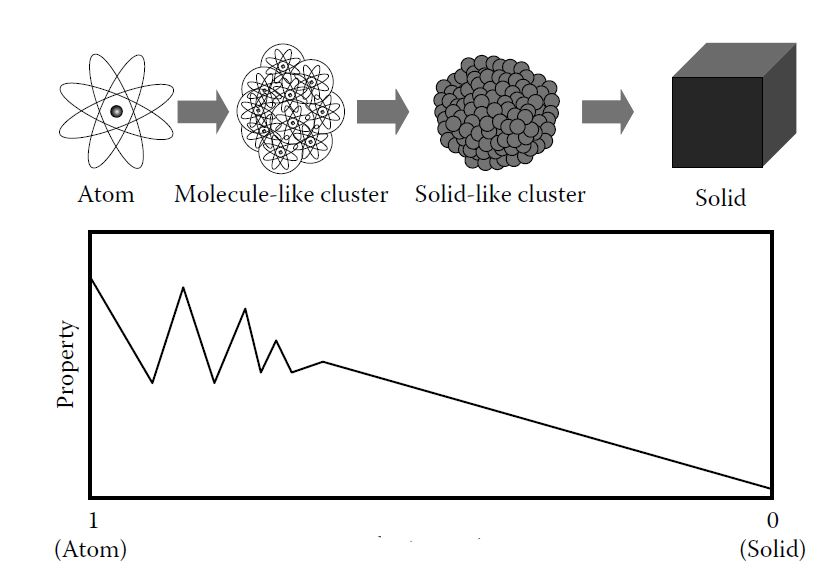
\includegraphics[width=0.8\textwidth]{images/clusters/atomo_cluste_solido}
  \caption{Esquema de transformação dimensional de átomos através de pequenos e grandes \textit{clusters} para o estado sólido. Quando os \textit{clusters} são pequenos cada átomo adicionado é importante, por isso as propriedades mudam
de forma abruptamente com o tamanho. Quando os \textit{clusters} se tornam grandes,
propriedades mudam suavemente\cite{cap06_Nanophysics}. Adaptado.  }
  \label{fig:transicao_cluster_solido}
\end{figure}

Uma das mudanças de propriedades interessantes é o surgimento de características semicondutoras em nanopartículas metálicas, que pode ser vista de Figura\ref{fig:carac_metal}. À medida que o número de átomos aumenta, também aumenta o número de níveis de energia disponíveis, até que a divisão entre níveis ocupados e desocupados se torna muito próxima e o \textit{cluster} começa a exibir comportamento metálico. Se aumentarmos um pouco o tamanho desta nanopartícula essas começaram a exibir comportamentos de pequenos pedaços do metal macroscópico. Abaixo desse tamanho crítico, os \textit{clusters} de elementos metálicos podem ter propriedades semelhantes a semicondutores.


\begin{figure}
  \centering
  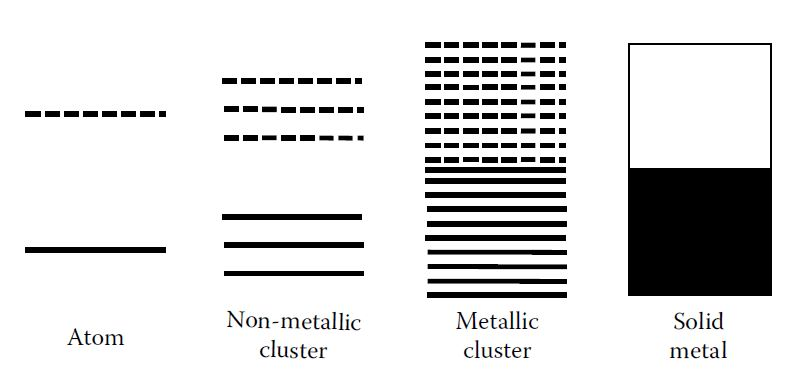
\includegraphics[width=0.7\textwidth]{images/clusters/carac_metal}
  \caption{ Esquema de transformação estrutural de energia a partir de átomos de metal através de pequenos e grandes \textit{clusters} para o metal sólido. Abaixo de um certo tamanho de \textit{clusters}, no qual as bandas vazia e povoada se fundem, um \textit{clusters} de átomos de metal pode ter uma estrutura de energia semelhante a um semicondutor.\cite{dissertacao_anderson}  }
  \label{fig:carac_metal}
\end{figure}



Deixando de lado os casos limites que geram ambiguidades, a diferença entre \textit{cluster} e moléculas encontra-se no fato que estas, no geral, possuem composições específicas e bem definidas e, na grande maioria dos casos, suas estruturas também são bem definidas, tendo  assim um número restrito de átomos; diferente um \textit{cluster}, como exemplo podemos citar um \textit{cluster} de prata que pode conter de 2, 15, 100, ou qualquer outro número de átomos de prata respeitando os limites impostos para que este ainda seja um \textit{cluster}. Esses por sua vez também não possuem uma estrutura única, como podemos ver na Figura \ref{fig:estrutura_cluster_ag}, e para sua maioria, à medida que o número de partículas do \textit{cluster} aumenta, o número de estruturas estáveis disponíveis torna-se mais abundante. 

\begin{figure}
  \centering
  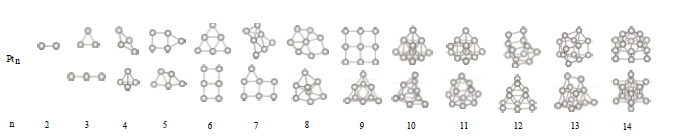
\includegraphics[width=1\textwidth]{images/clusters/estrutura_cluster_ag}
  \caption{ Exemplo de estruturas de \textit{clusters} de prata.\cite{dissertacao_anderson}  }
  \label{fig:estrutura_cluster_ag}
\end{figure}


O histórico de estudo da organização espacial dos arranjos atômicos frutificou em um Prêmio Nobel de Física em 1963. Metade do prêmio foi dado a Eugene Paul Wigner, por sua contribuição para a teoria do núcleo atômico e as partículas elementares,  e a outra metade foi partilhada por Maria Goeppert Mayer e J. Hans D. Jensen, pelas suas descobertas relativas à estrutura da casca nuclear. A análise das estruturas dos \textit{clusters} é fundamental para compreender suas propriedades e  dispor de seus potenciais tecnológicos, isso também torna-se muito importante para o domínio da estabilidade das nanopartículas. 



Em 1984, Knight et al \cite{electronic_Shell_sodium}, realizou um experimento com nanopartículas de sódio (Na), com N átomos por conglomerado (N = 4-100), e foram encontrado padrões, com picos bem definidos, no espectro de massa de \textit{clusters} de Na em fase gasosa, podendo ser visto na Figura \ref{fig:espec_na}(a). Cada pico do espectro representa o número de 
aglomerados de um determinado N detectado. Note a presença de picos maiores, quando comparado com os outros picos, para certas massas correspondentes à N = $8, 20, 40, 58$ e $92$, onde podemos notar padrões. Os \textit{clusters} mais abundantes
no espectro de massa são considerados relativamente mais estável. Podemos destacar a estrutura eletrônica dessas nanopartículas como a causa de maior estabilidade. Esses picos foram apelidados de \textit{clusters mágicos} ou \textit{clusters com números mágicos de átomos}.




\begin{figure}
  \centering
  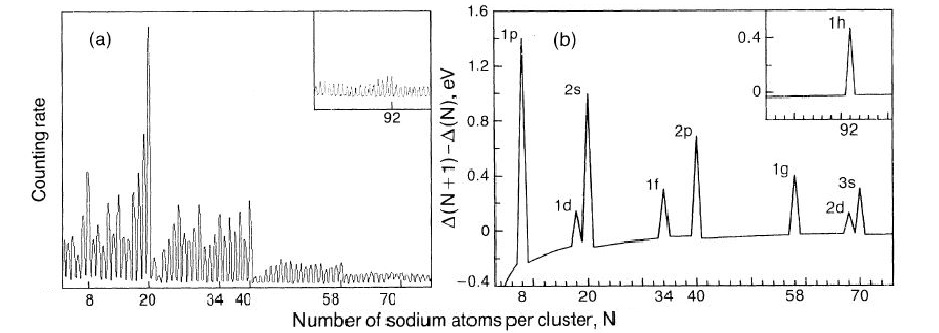
\includegraphics[width=1\textwidth]{images/clusters/NA_knight}
  \caption{(a) Espectro de massa de \textit{clusters} de sódio, N = 4-75.
  (b) A mudança calculada na diferença de energia eletrônica. Os picos protuberantes correspondem aos orbitais de casca fechada.\cite{electronic_Shell_sodium}  }
  \label{fig:espec_na}
\end{figure}


Podemos explicar a ocorrência desses \textit{clusters mágicos} foi suposto o efeitos de preenchimento de camadas eletrônicas, em que a combinação entre o espectro de estados
quantizados e o princípio de exclusão de Pauli resulta em efeitos de camada \cite{Brack}.O modelo quântico de \textit{Jellium} \cite{Heer}, foi usado com sucesso para explicar a ocorrência desses \textit{clusters mágicos} \cite{capitulo_livro_shell}.

As características dos espectros de massa de outros metais alcalinos e também dos metais nobres, seguem um padrão semelhante ao do sódio. Para as nanopartículas consideradas grandes, o padrão de números mágicos aparece diferente, e no geral ele é atribuído como uma consequência do preenchimento de camadas geométricas ou poliédricas de casca, assim o \textit{clusters} assume geometrias que minimizam a relação átomo-superfície uma vez que os átomos da superfície possuem um número menor de vizinhos do que os átomos internos, e o \textit{clusters} tende a preferir a estrutura de menor energia, maximizando a fração de átomo em massa. Essa estrutura geométrica da casca é bem conhecida nos \textit{clusters} de gás, e é característica de interações de curto alcance nas quais a tendência é para o empacotamento próximo do atomizado juntamente com a necessidade de minimizar a energia superficial \cite{capitulo_livro_shell}.




\section{Estrutura eletrônica \textit{shell model} para \textit{clusters} esféricos} \label{section_shell_model}

Pretendemos apresentar uma visão geral das características do sistema eletrônico \textit{shell model}.

O espectro de de massa da \ref{fig:espec_na} sugere que, os elétrons de valência nos \textit{clusters} de sódio são independentes e estão confinados em um potencial esfericamente simétrico. Assim como os átomos, as camadas eletrônicas de um \textit{cluster} com um número exato de elétrons para formar uma estrutura geometria poliédrica fechada, é muito estável. Assim que um átomo for adicionado a nanoestrutura, seu elétron de valência ocupará um estado com energia maior e assim a estabilidade do \textit{cluster} será reduzida, ocasionando uma rejeição deste estado e reduzindo sua sua abundância no espectro e isso explica a grade abundância após cada número de fechamento da casca.

Os números quânticos dos \textit{cluster} metálicos, são caracterizados de modo que cada casca é possuí um número quântico radial \textit{n} e o momento angular \textit{l}. Para um dado número quântico \textit{l}, o estado mais baixo tem $n = 1$, e assim por diante.


Uma abordagem com respaldo na mecânica quântica e que fornece uma descrição boa do comportamento observado na Figura \ref{fig:espec_na}, é considerarmos um elétron se movendo em um campo médio onde calculamos considerando que eles são partículas independentes movendo-se em um potencial parametrizado. O parâmetro básico do modelo é o raio de Wigner-Seitz, $r_{s}$, o raio de uma esfera contendo um elétron. O raio de um átomo de \textit{N} (ou elétron de valência) é dado por:

\begin{equation}
    R = r_{s}(N)^{\frac{1}{3}}
\end{equation}

É útil considerar a estrutura eletrônica surgindo com alguns potenciais simples. Para potenciais simétricos esfericamente, a função de onda é separável em uma parte radial e angular:

\begin{equation}
    \psi_{ n,l,m}(r, \theta, \phi) = R_{nl}(r)Y_{lm}(\theta, \phi)
\end{equation}

com os números quânticos familiares e $2(2l+1)$ de degenerescência (incluindo spin) em relação a \textit{m}. Três potenciais úteis para o estudo da física de \textit{cluster}, são os harmônicos, o poço quadrado e os potenciais Woods-Saxon mostrados na Figura \ref{fig:pocos}.

O potencial mais simples é o potencial do oscilador harmônico $V_{r}$:

\begin{equation}
    V(r)= \frac{1}{2}m\omega_0r^2
\end{equation}

o potencial do poço quadrado esférico (constante para $r<R$ e infinito para os demais). Como podemos ver na primeira coluna da Figura \ref{fig:pocos} os níveis de energia para o potencial do oscilador harmônico são igualmente espaçados, altamente degenerados e são rotulados pelo número quântico \textit{v}.

\begin{equation}
    E_{v}= \left(\frac{3}{2}+v\right)h\omega_0
\end{equation}


\begin{figure}
  \centering
  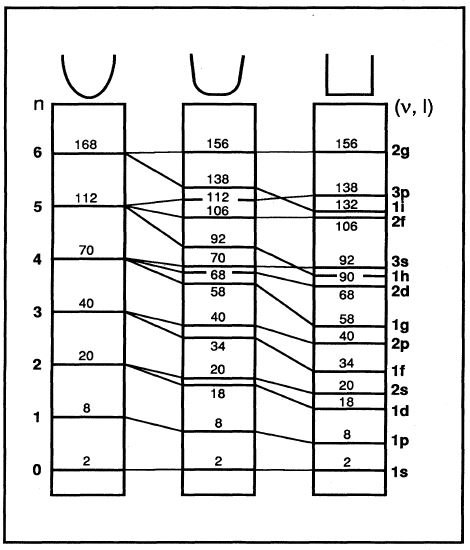
\includegraphics[width=0.5\textwidth]{images/clusters/pocos}
  \caption{(a) Espectro de massa de \textit{clusters} de sódio, N = 4-75.
  (b) A mudança calculada na diferença de energia eletrônica. Os picos protuberantes correspondem aos orbitais de casca fechada.\cite{electronic_Shell_sodium}  }
  \label{fig:pocos}
\end{figure}



\chapter{A fonte de \textit{clusters} e agregados}
\label{c3}

O objetivo deste capítulo é apresentar a máquina, desenvolvida por Artur Domingues Tavares de Sá e Giulia Di Domenicantonio \cite{tese_artur}, utilizada para a produção de nanopartículas de prata, estudadas neste trabalho.

\section{FoCA}

A Fonte de \textit{Clusters} e Agregados (FoCA), esquematizada na Figura \ref{fig:esquema_foca}, produz nanopartículas metálicas que variam entre $1$ podendo chegar $40.000$ átomos (ou $5nm$, no caso da prata), essa produção se da por método físico, mais especificamente \textit{sputtering}.

O funcionamento da máquina ocorre basicamente em quatro etapas: primeiramente uma nuvem de átomos é produzida por um \textit{sputtering}; em seguida, são resfriadas por nitrogênio líquido ocorrendo a agregação dos átomos em nanopartículas na presença do gás argônio; na sequência, o feixe de agregados, carregados eletricamente, é guiado por um conjunto de lentes eletrostáticas até chegar no espectrômetro de massa por tempo de voo, onde $\approx10\%$ do feixe é desviado para a análise do espectro de distribuição de massa, sendo possível identificar a massa e por consequência o tamanho das partículas produzidas, por fim as nanopartículas são depositadas no porta amostras. Na Figura \ref{fig:foto_foca} podemos ver uma foto real da máquina. 

\begin{figure}
  \centering
  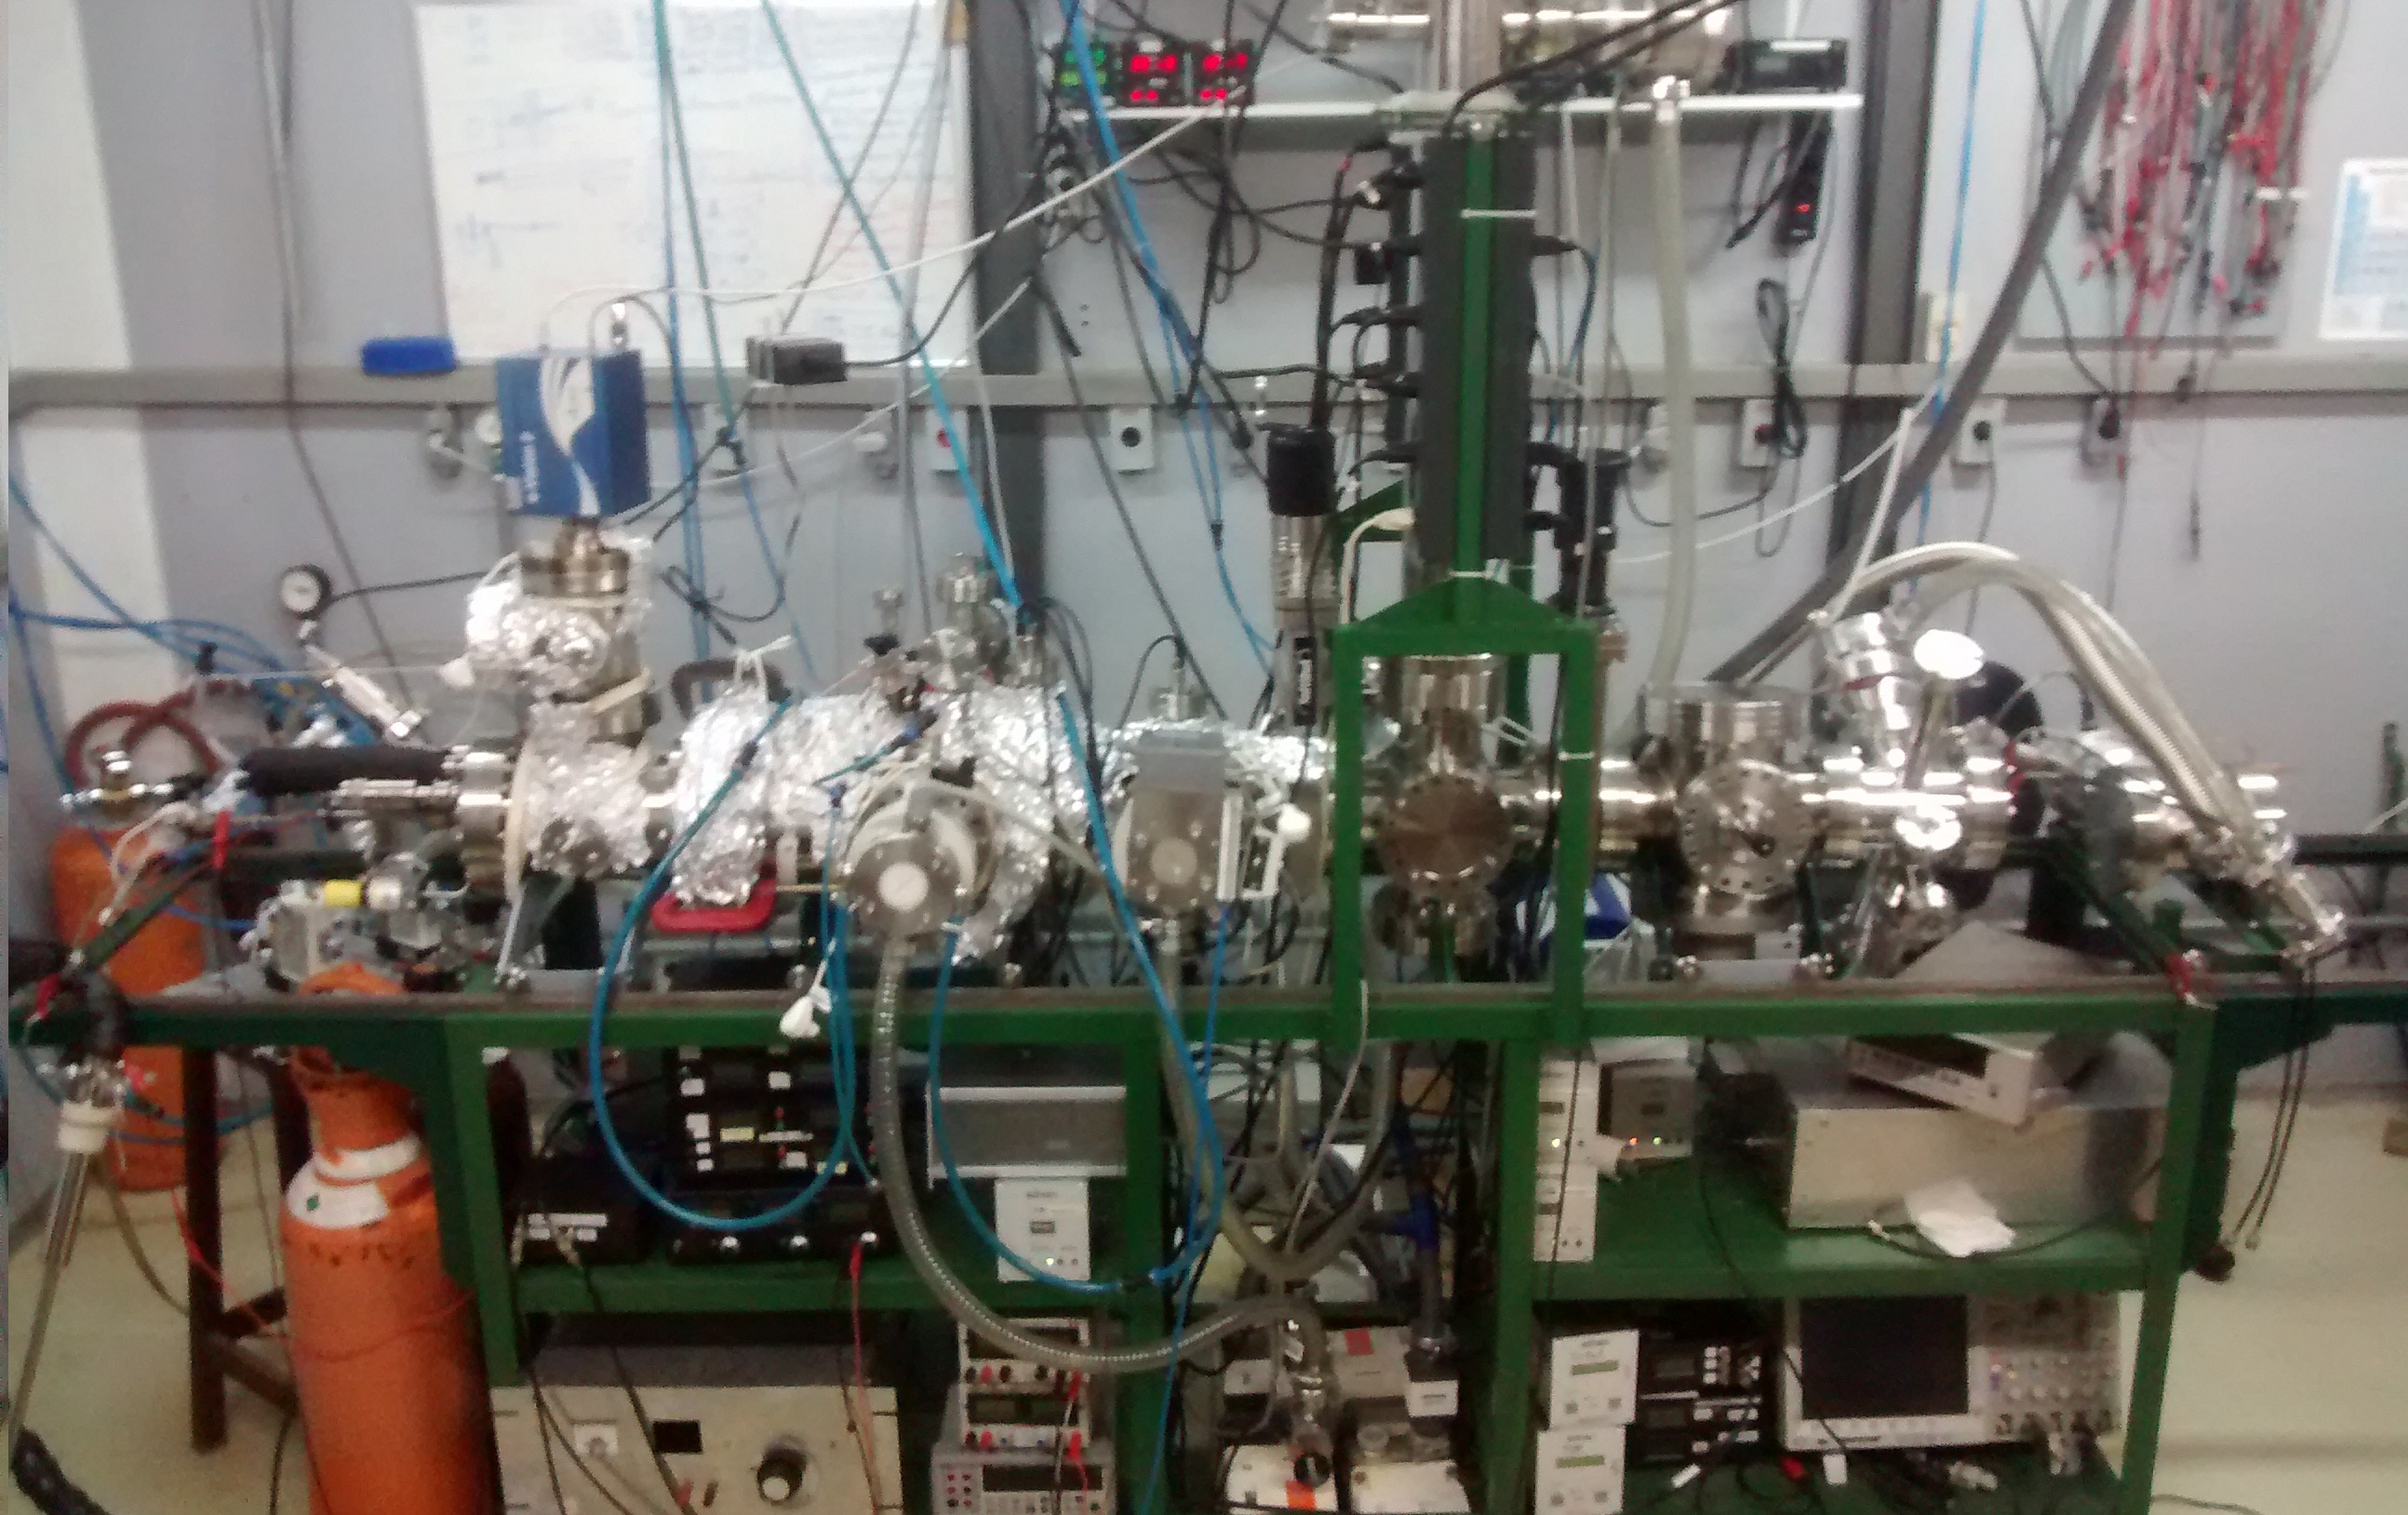
\includegraphics[width=0.7\textwidth]{images/foca/foto_foca}
  \caption{ Imagem real da  Fonte de \textit{Clusters} e Agregados.  }
  \label{fig:foto_foca}
\end{figure}

\begin{figure}
  \centering
  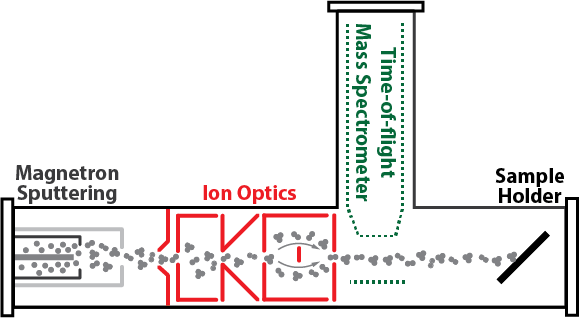
\includegraphics[width=0.8\textwidth]{images/foca/esquematico_foca}
  \caption{ Diagrama da fonte de Fonte de \textit{Clusters} e Agregados. ``\textit{Magnetron Sputtering}'' é a fonte de átomos que se encontra dentro da câmara de agregação. Depois de produzido e agregado, o feixe passa por um conjunto de lentes eletrostásticas  ``\textit{Ion Optics}''. Uma parte do feixe é desviado para o ``\textit{Time-of-flight Mass Spectrometers}'' (ToF), onde é realizada a aquisição do espectro de voo, outra parte é depositada na amostra "\textit{Sample Holder}"\cite{livro_vitor}.  }
  \label{fig:esquema_foca}
\end{figure}

As lentes eletrostáticas possuem as seguintes funções: focalizar o feixe de íons, retirar as partículas neutras, de acordo com o potencial aplicado nas lentes elas também podem funcionar com um filtro em função das energias das partículas. As lentes consistem de uma série de eletrodos de simetria cilíndrica nas quais são aplicadas potenciais. Uma foto das lentes pode ser vista na Figura \ref{fig:foto_lentes}.

\begin{figure}
  \centering
  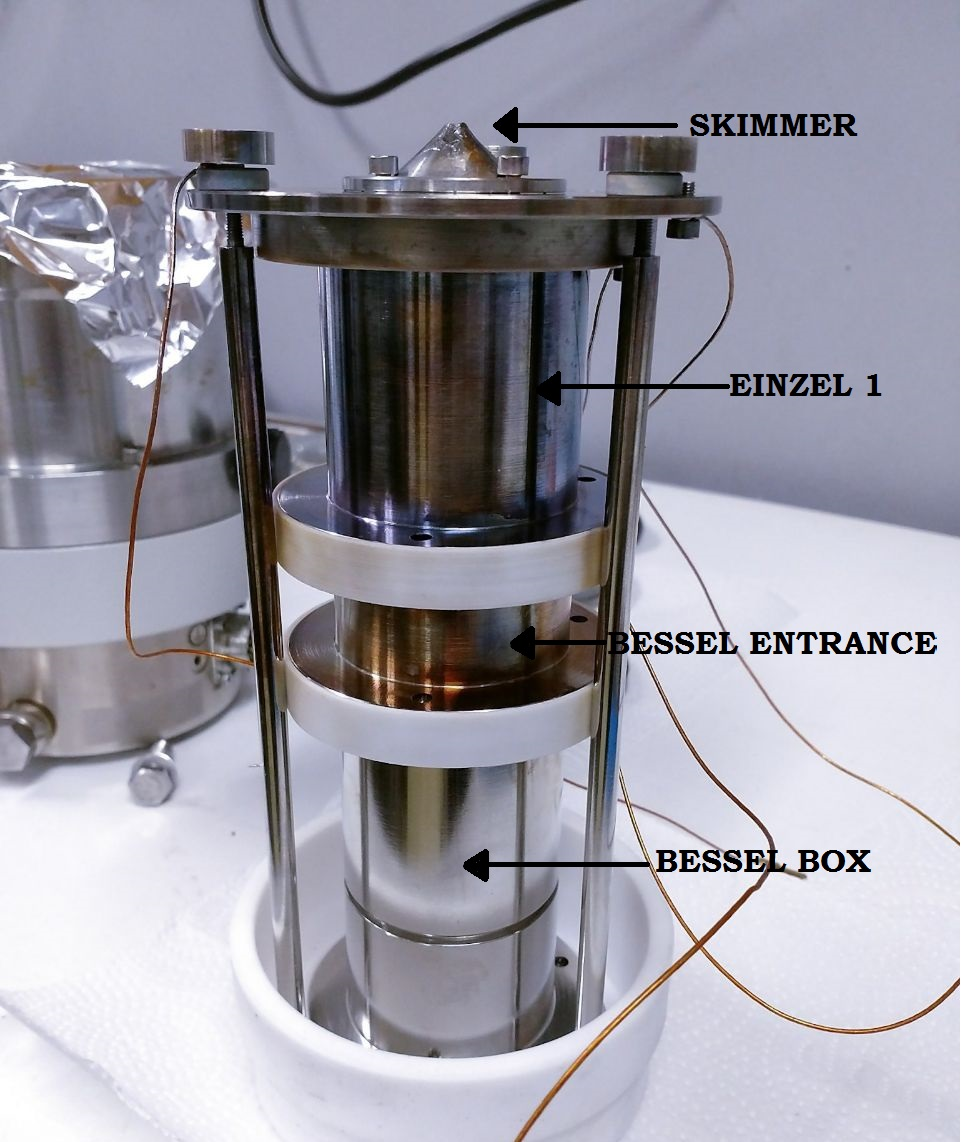
\includegraphics[width=0.6\textwidth]{images/foca/lentes}
  \caption{ Foto da lentes eletrostáticas.  }
  \label{fig:foto_lentes}
\end{figure}



Existem muitas formas de síntese de nanopartículas, seja por método químico ou físico. Como exemplo da primeira, para o caso da prata, podemos citar a redução com borohidreto de sódio e como exemplo da segunda, agora em um caso mais geral de metais, podemos citar a evaporação térmica e a técnica de \textit{sputtering} ou pulverização catódica.

Para gerar nossa nuvem de átomos, a FoCA utiliza um \textit{magnetron cilíndrico} \cite{ref_artigo_foca}, que caracteriza a produção desses \textit{clusters} por \textit{sputtering}, aqui o alvo, material que dará origem às nanopartículas, possuí o formato de um fio e fica localizado no eixo do \textit{magnetron}.

A versatilidade dessa técnica encontra-se no fato que o alvo é multivalente, podendo ser composto de vários metais, incluindo ligas, como por exemplo a mistura ouro e prata, bastando entrelaçar os fios do metal de desejo para isso. Na Figura \ref{fig:magnetron} podemos ver o plasma gerado no \textit{magnetron cilíndrico}. Pela presença de um campo elétrico os íons são acelerados em direção ao alvo do metal de interesse e o corrói. Na Figura \ref{fig:alvo} é possível observar um alvo de prata, composto por um único fio, novo e ao lado um já erodido.

\begin{figure}
  \centering
  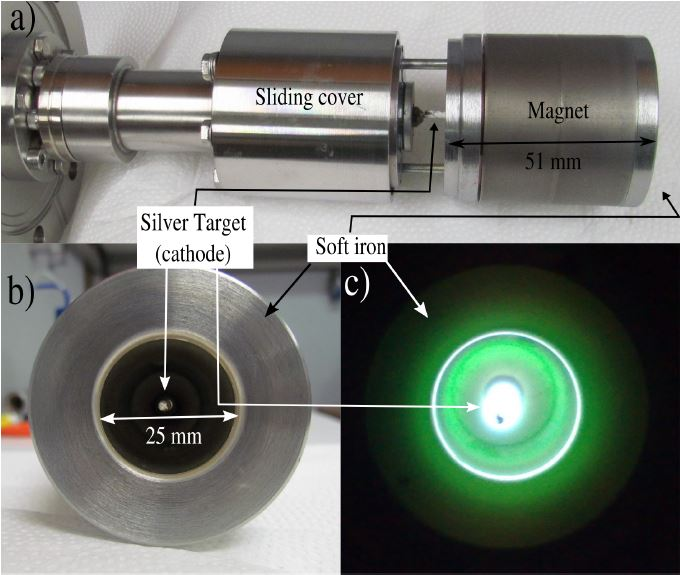
\includegraphics[width=0.75\textwidth]{images/foca/magnetron_cil}
  \caption{ (a) Magnetron cilíndrico oco caseiro com a tampa deslizante retraída para mostrar o alvo de prata. (b) vista frontal. (c) Vista frontal com plasma aberto. Observe a cor esverdeada ao redor do alvo, tipicamente vista na formação de plasma prateado.\cite{livro_vitor} }
  \label{fig:magnetron}  
\end{figure}


\begin{figure}
  \centering
  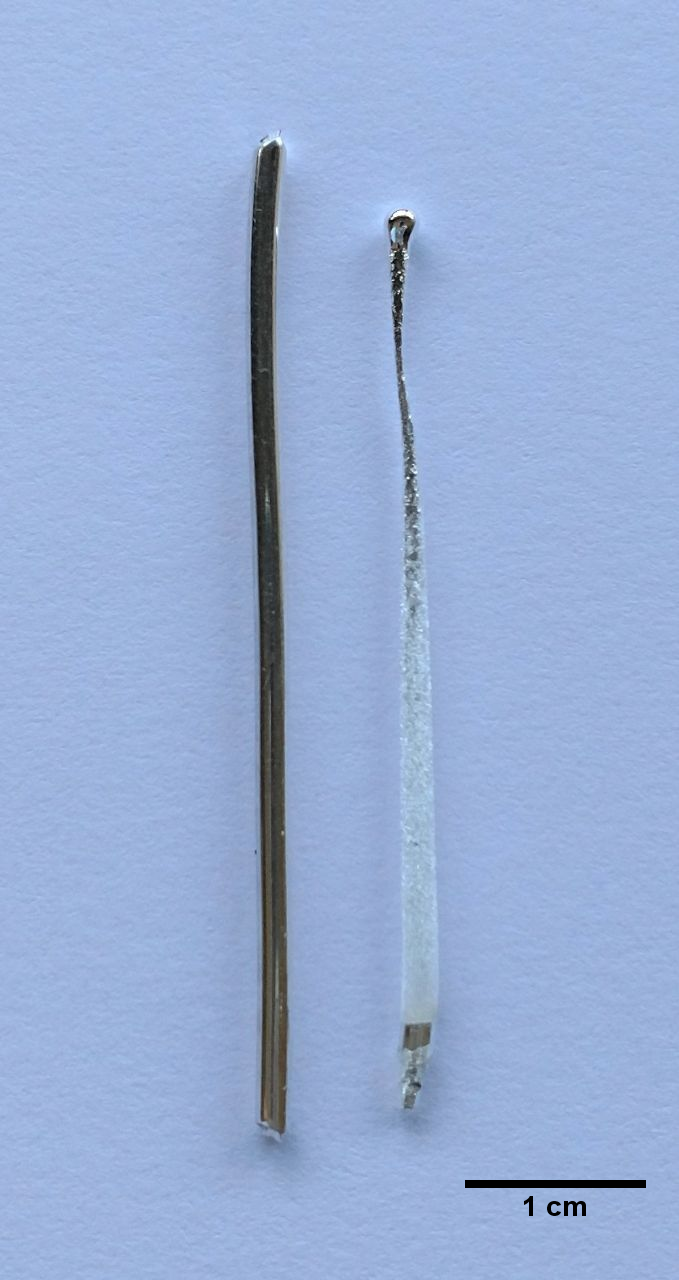
\includegraphics[width=0.3\textwidth]{images/foca/alvo}
  \caption{ Foto de um alvo de prata de fio único. À esquerda temos um alvo novo e à direita temos um alvo já corroído.  }
  \label{fig:alvo}
\end{figure}






\section{Espectrômetro de massa por tempo de voo}

Esta seção será dedicada a descrever o princípio de funcionamento da técnica de \textit{Time-of-flight Mass Spectrometers} (TOFMSs).

Na Figura \ref{fig:tof}, pode-se observar o esquema do espectrômetro, onde o pulso elétrico fornece velocidade perpendicular ao feixe de partículas carregadas, que viajam dentro de um tubo de voo - livre de variação de potencial elétrico - até encontrarem um detetor de corrente. Por sua vez, o detetor faz a contagem de íons em função dos tempos de chegada.

O TOFMSs funciona  baseado no fato de que, ao receber a mesma quantidade de energia fornecida por um campo elétrico pulsado, partículas com massas diferentes adquirem velocidades distintas \cite{dissertacao_kevin}. Assim, as partículas mais leves atingirão o detector antes das partículas mais pesadas.

\begin{figure}
  \centering
  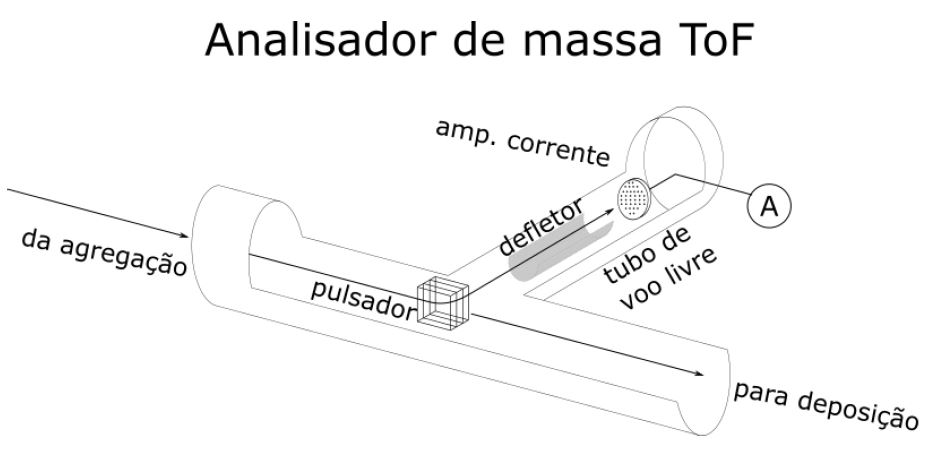
\includegraphics[width=1\textwidth]{images/foca/tof}
  \caption{ O pulsador é um conjunto de placas com campo pulsado, que confere uma velocidade perpendicular ao feixe de partículas eletricamente carregadas. Os defletores impedem que as partículas colidam com as paredes do tubo de voo livre. ``\textit{A}'' representa o detector de corrente, cuja função é realizar a contagem dos íons em função do tempo de chegada.  \cite{dissertacao_kevin}.  }
  \label{fig:tof}
\end{figure}

Para calcular o tempo de voo, vamos considerar um \textit{cluster} de massa $m$ e carga $q$. O campo elétrico vai fornecer energia cinética ($K = qV$) para a partícula, em que $V$ é a voltagem fornecida pelo pulsador. Assim, é possível expressar a velocidade da partícula como:

\begin{equation}
v = \sqrt[]{\frac{2qV}{m}}
\end{equation}

O detector de corrente está situado a uma distância $L$ da região onde a partícula adquire velocidade. Note que essa partícula levará um tempo $t_{voo}$ para atingir o detector, e esse tempo pode ser calculado por:

\begin{equation}
\label{eq:tempo_voo}
t_{voo} = L \cdot \sqrt[]{\frac{1}{2V} \frac{m}{q}} 
\end{equation}


A corrente que chega ao detector é convertida em tensão por um amplificador IV, e o sinal é exibido em um osciloscópio, e então para aquisição dos dados utiliza-se um programa desenvolvido pelo grupo.

A variável $L$ possui o valor de um metro, o potencial aplicado é de $V = 7 $  kV, e o tempo de voo das partículas é fornecido pelo osciloscópio, possibilitando calcular a massa das partículas.

Note que utilizando a Equação \ref{eq:tempo_voo} é possível também calcular o $t_{voo}$ de uma partícula se soubermos a massa. Vamos fazer uma análise para o caso de um átomo de prata. Segundo a tabela periódica um átomo de prata possui uma massa de $107,87$ unidades de massa atômica, convertendo sua massa para quilos temos $1,79\times 10^{-25}$ kg. A carga de partícula é a carga elementar de um elétron $1,60\times 10^{-19}$ C, e então seu tempo de voo vai ser aproximadamente$17,6$ $\mu$s.

Podemos também escrever a massa de uma nanopartícula em função da massa de uma outra partícula da qual conhecemos a massa e o tempo de voo.

\begin{equation}
\label{eq:relacao_massa_tempo}
M = \left(\frac{t}{t'}\right)^2 \cdot M'
\end{equation}


É possível estabelecer uma relação que futuramente vai permitir diferenciar outros picos de prata, e então calibrar o espectro de partículas produzido, confirmando o que foi depositado na amostra.


A grande vantagem desse tipo de técnica, espectrometria de massa por tempo de voo, é que a obtenção da distribuição de tamanhos produzida é exibida em tempo real, assim qualquer deformidade indesejável no espectro é passível de correção ainda durante o processo de deposição, por meio de ajuste  dos parâmetros da máquina. 

\section{Experimentos com luz ultravioleta}

Para realizar experimentos com incidência de luz ultra violeta, foi preciso montar um sistema de iluminação, que consiste em inserir um LED do UV, modelo UVTOP240 TO39 produzido pela Roithner Lasertechnik GmbH, na fonte de agregados. Para isto foi instalado um passante de tensão para que o LED fique em dentro da máquina. Além disso, um sistema de alimentação, com controle de corrente, foi montado utilizando uma fonte de tensão.

O LED é baseados em AlGaN (Alumínio, Gálio e Nitrogênio), com um pico típico de comprimento de onda de $245 nm$ e potência de saída óptica de $30-70 \mu W$. Seu encapsulamento é metálico e hermeticamente fechado, com configuração de lente de vidro plano. Uma foto desse diodo pode ser vista na Figura \ref{fig:foto_led}.

\begin{figure}
  \centering
  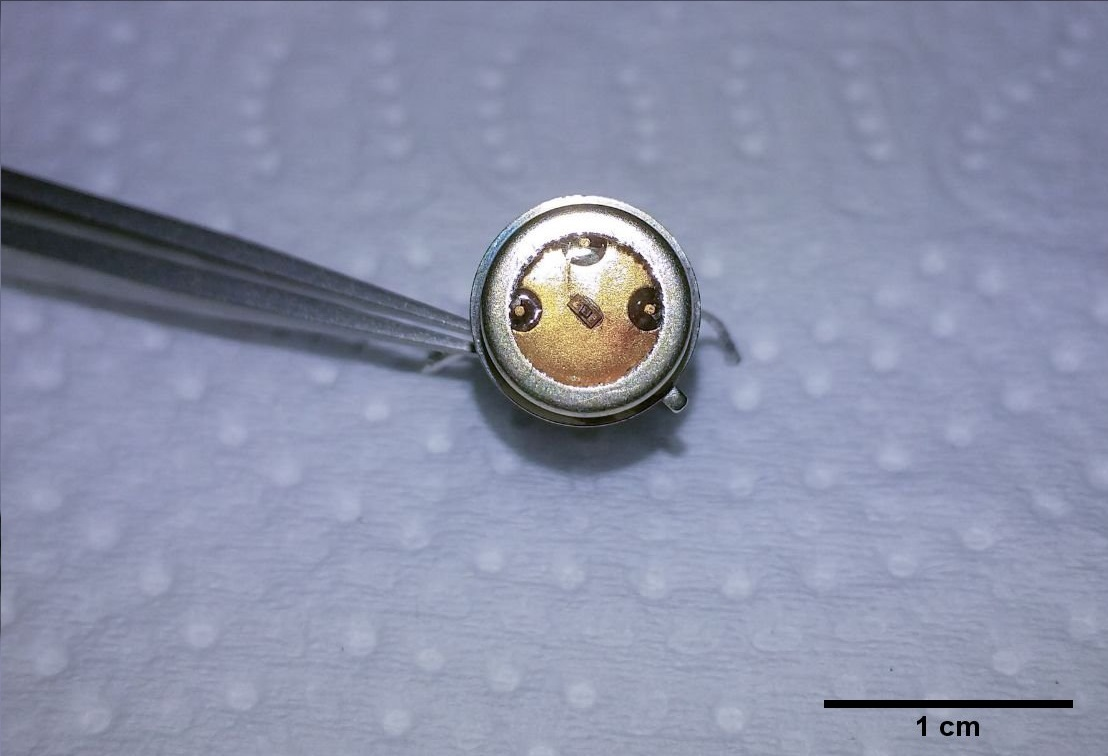
\includegraphics[width=0.7\textwidth]{images/foca/led_scale}
  \caption{ Foto do LED do UV, modelo UVTOP240 TO39, utilizado para ionização das nanopartículas.  }
  \label{fig:foto_led}
\end{figure}


Foi escolhido posicionar o LED entre saída da câmara de agregação e a primeira lente eletrostática, como podemos ver na Figura \ref{fig:led_montagem}. Os testes do aparato consistem na aquisição da corrente de agregados produzidos e do seu espectro de massa sem o uso do LED e posteriormente com o LED. Com isso foi avaliado o possível aumento de ionização, como a incidência de luz afeta o espectro de massa do sistema de agregação e possíveis ajustes nos valores da tensões das lentes eletrostáticas.
Assim, foram realizados experimentos com incidência de luz ultra violeta (UV), induzindo a sua ionização, e comparar os espectros de abundância obtidos com e sem o uso da luz UV. 



\begin{figure}
  \centering
  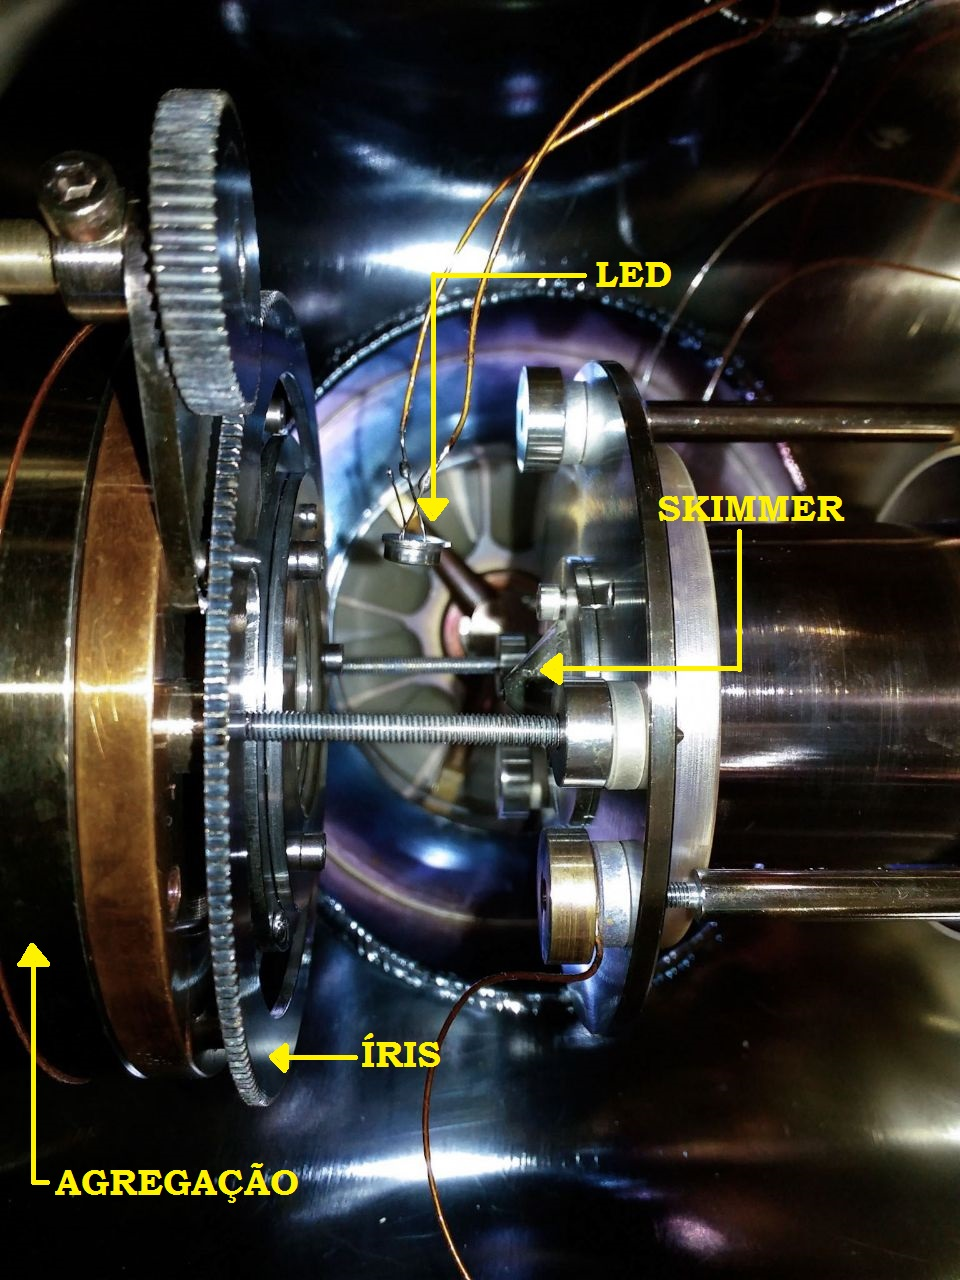
\includegraphics[width=0.7\textwidth]{images/foca/led_montagem}
  \caption{Foto do posicionamento do LED, localizado entre a câmara de deposição e a primeira lente eletrostática, Skimmer. Também está indicado a íris, peça que controla a pressão na câmara de agregação.}
  \label{fig:led_montagem}
\end{figure}





\chapter{Capítulo com muitas fórmulas} \label{ometodo}

Neste capítulo realizaremos uma detalhada descrição do método de DMC na seção \ref{alg_padr}. ....

\section{O algoritmo padrão}
\label{alg_padr}

Se escrevemos a equação de Schroedinger,

\begin{equation} \label{eschrodinger}
i\hbar \frac{\partial \Psi}{\partial t}= -\frac{\hbar^2}{2m}
\nabla_R^2 \Psi + V\Psi,
\end{equation}

\noindent em tempo imaginário ($\tau=it/\hbar$), vemos que esta
pode ser interpretada como uma equação de difusão da forma

\begin{equation} \label{eischrodinger}
\frac{\partial \Psi}{\partial \tau}= D \nabla_R^2 \Psi - V
\Psi = - H \Psi,
\end{equation}

\noindent onde $D=\hbar^2/2m$ é a constante de difusão.

Mediante esta transformação, as soluções gerais da equação
(\ref{eschrodinger}) são
modificadas para a forma

\begin{equation} \label{solim}
\Psi({\bf R},\tau) = \sum_i \phi_i ({\bf R}) \exp  \left( - E_i
\tau \right),
\end{equation}

\noindent onde $\phi_i$ e $E_i$ são as funções e valores próprios
respectivamente da equação de Schroedinger independente do tempo.
Notemos que o fato de utilizarmos tempo imaginário transforma a
solução (\ref{solim}) em uma soma de termos exponenciais decrescentes. Como uma
constante
$E_T$ pode ser
introduzida na energia potencial do sistema sem modificar a forma
funcional das
autofunções $\phi_i({\bf R})$, a equação (\ref{eischrodinger}) e a
sua solução
(\ref{solim}) podem ser reescritas como:

\begin{equation} \label{eqsch2}
\frac{\partial \Psi}{\partial \tau}= D \nabla_R^2 \Psi -
(V-E_T) \Psi = -H \Psi
\end{equation}

\noindent e

\begin{equation} \label{solim2}
\Psi({\bf R},\tau) = \sum_i \phi_i ({\bf R}) \exp  \left( -
(E_i - E_T) \tau
\right);
\end{equation}

\noindent onde a Hamiltoniana do sistema é dada agora por $H =
T+(V-E_T)$. Como
consequência disto, para uma evolução temporal longa o suficiente da
solução
$\Psi({\bf R},\tau)$
(\ref{solim2}), e ajustando adequadamente o valor da constante
$E_T$, o único estado sobrevivente é o fundamental. Pode-se
dizer então que a evolução do sistema no tempo
imaginário projeta o sistema no seu estado fundamental.

A equação (\ref{eqsch2}) possui uma solução formal do tipo

\begin{equation} \label{esimpli}
|\Psi(\tau)\rangle = G |\Psi^{'}(0)\rangle,
\end{equation}

\noindent onde $G = \exp(-\tau H)$. Integrando a equação (\ref{esimpli}) 
obtemos a
seguinte expressão

\begin{equation} \label{intpsi}
\Psi({\bf R},\tau) = \int {\bf dR}^{'} G({\bf R^{'}} \rightarrow
{\bf R}, \tau) \Psi({\bf R}^{'}, 0),
\end{equation}

\noindent com a qual podemos evoluir uma representação da função de onda do 
sistema em um
intervalo de tempo
$\triangle \tau$. A função de Green $G({\bf R}^{'}
\rightarrow {\bf R}, \tau)$ da equação (\ref{intpsi}) pode ser
interpretada
como a probabilidade de transição das partículas da
posição
${\bf R}^{'}$ para
${\bf R}$ num tempo $\tau$. A representação da função de Green
$G({\bf R}^{'}
\rightarrow {\bf R}, \tau)$ no espaço das coordenadas é dada por

\begin{equation} \label{funcaogreen}
G({\bf R}^{'} \rightarrow {\bf R}, \tau) = \langle {\bf
R}|\exp[-\tau \hat{T} -
\tau (\hat{V} - E_T)]|{\bf R}^{'} \rangle,
\end{equation}

\noindent onde $\hat{T}$ e $\hat{V}$ são os operadores da energia
cinética e
potencial respectivamente. Como notação, a
função de Green
(\ref{funcaogreen}) vai ser representada por $G(R,R^{'})$.

Em geral, o cálculo da função $G(R,R^{'})$ não é tarefa fácil mas
pode ser
simplificada se usarmos a chamada aproximação de tempo pequeno
(``short-time
aproximation''). Isto implica expandir o comutador da função de
Green da equação
(\ref{funcaogreen}) para tempos pequenos. Realizando isto se obtém
uma forma da função de Green dada por

\begin{eqnarray} \label{gaprox}
G(R,R^{'}) &\cong& \langle {\bf R}|\exp(-\triangle \tau
\frac{\hat{V}}{2})
\exp(-\triangle \tau \hat{T}) \exp(-\triangle \tau
\frac{\hat{V}}{2})|{\bf
R}^{'}\rangle \nonumber \times \\ &&
\exp(\triangle \tau E_T) \nonumber \\ &=&
\exp(-(\frac{\triangle\tau}{2})\{V(R) +
V(R^{'})\} + \triangle\tau E_T) \nonumber \times \\ && \langle
{\bf R}|
\exp-(\triangle\tau \hat{T})|{\bf R}^{'} \rangle \nonumber \\ &=&
G_b(R,R^{'})
G_d(R,R^{'}).
\end{eqnarray}

\noindent Aqui $G_d(R,R^{'})$ é a solução ordinária da equação da
difusão e
$G_b(R,R^{'})$ pode ser interpretada como a razão de decaimento ou 
crescimento associada à configuração $R$ das partículas.
Explicitamente estas funções são
dadas respectivamente por

\begin{equation} \label{greenb}
G_b(R,R^{'}) = \exp(- (\frac{\triangle\tau}{2}) [V(R) + V(R^{'})]
+ \triangle\tau
E_T)
\end{equation}

\noindent
e

\begin{equation} \label{greend}
G_d(R,R^{'}) = (4 \pi D \triangle\tau)^{-\frac{3N}{2}}
\exp[-\frac{({\bf R} - {\bf
R}^{'})^2}{4D\triangle\tau}].
\end{equation}

É importante mencionar que a expressão da função de Green (\ref{gaprox}) é correta só
até ordem
O($\tau^3$). Isto implica que para obter resultados 
exatos, devemos usar
intervalos de tempo $\triangle\tau$ pequenos e
realizar uma extrapolação dos resultados para $\triangle \tau \rightarrow
0$ (veja entretanto comentários no Capítulo \ref{asimulação}). O valor de 
$\triangle \tau$ é um
parâmetro
em nossos cálculos.

Um conjunto inicial de configurações é propagado por um
intervalo de tempo
$\triangle\tau$ mediante o uso da
função de Green $G(R,R^{'})$
(\ref{gaprox}). Isto é feito através dos processos
de difusão e
``branching''. Para difundir as configurações é preciso aplicar a
função $G_d(R,R^{'})$ (\ref{greend})
sobre cada uma das partículas de cada configuração. Isto se reduz a
deslocar cada uma das
coordenadas das partículas, por exemplo $x$, de acordo com

\begin{equation}
x = x^{'} + \chi \; ,
\end{equation}

\noindent onde $\chi$ é um número aleatório amostrado de uma
Gaussiana de variança
$2D\triangle\tau$ e média zero. Neste caso temos que fazer $3N$ atualizações das
posições das partículas
para propagar uma
configuração, sendo $N$ o número de partículas do sistema. Alternativamente, é
possível deslocar todas as partículas simultaneamente com pequenas modificações no
algoritmo.

Inicialmente cada uma das configurações começa a sua evolução
carregando um peso
$w^{'}$ igual a um. Após a evolução de cada uma das configurações, os pesos destas
são atualizados usando a função $G_b(R,R^{'})$ (\ref{greenb}). Estes pesos são
atualizados de acordo com:

\begin{equation} \label{atpesos}
w=w^{'}G_b(R,R^{'}).
\end{equation}

Após a propagação de todas as configurações chegamos a uma nova
geração. Neste momento é possível realizar uma
amostragem da função de onda $\Psi(R,\tau)$. Por motivos de
eficiência, a quantidade
de configurações usadas para estimar $\Psi(R,\tau)$ varia, este
é o chamado processo
de ``branching''; o qual será explicado na Seção seguinte.

\section{Amostragem de importância}

Existem vários problemas associados ao método como implementado na seção anterior.
Um deles surge do
fato de que para certos potenciais (como o potencial de Coulomb) a
função
$G_b(R,R^{'})$ aumenta muito o número das configurações quando
as partículas estão
muito próximas, já que $V(r) \rightarrow -\infty$.
Outro problema prático com relação ao
método surge do fato que as partículas podem perder muito tempo navegando 
por
regiões do espaço
de configuração que não são relevantes para o cálculo final. Para
eliminar estes problemas, se multiplica a equação de Schroedinger da equação 
(\ref{eqsch2}) por uma
função $\Psi_G$ conhecida, que aproximadamente representa o
estado
fundamental do sistema. Este procedimento é chamado de
amostragem de importância. Uma vez feito isto, a equação de Schroedinger em 
tempo
imaginário
(\ref{eqsch2}) pode ser reescrita como

\begin{equation} \label{eresschroedinger}
\frac{\partial f}{\partial \tau} = D \nabla_R^2 f - D
\nabla_R \cdot [f{\bf F}] + [E_T - E_L({\bf R})] f,
\end{equation}

\noindent onde $f=\Psi_G\Psi$, $E_L({\bf R})={H \Psi_G}/{\Psi_G}$ e ${\bf 
F}=
2\nabla_R \ln
\Psi_G$. Neste caso $E_L$ é a energia local do sistema e a função
${\bf F}$ atua como
uma força de arraste imposta na difusão. A presença da função
${\bf F}$ na equação
(\ref{eresschroedinger}) permite que as partículas sejam
arrastadas para regiões do
espaço onde $f$ é importante.

Para resolver a equação (\ref{eresschroedinger}) notemos que sua
função de Green
satisfaz

\begin{equation}
\frac{\partial \tilde{G}}{\partial \tau} = - \tilde{H}\tilde{G} =
- (\tilde{T} +\tilde{V}) \tilde{G},
\end{equation}

\noindent onde o operador $\tilde{T}$ é dado por

\begin{equation}
\tilde{T}= - D \nabla_R^2 + D  \nabla_R \cdot {\bf F}+ D
{\bf F} \cdot \nabla_R
\end{equation}

\noindent e $\tilde{V}$ como

\begin{equation}
\tilde{V} = E_L - E_T.
\end{equation}

\noindent Desta forma, e utilizando a aproximação de tempos pequenos, 
podemos
escrever a função de Green do sistema como

\begin{equation} \label{fgreen2}
\tilde{G}(R,R^{'})= \tilde{G}_b(R,R^{'}) \tilde{G}_d(R,R^{'}),
\end{equation}

\noindent onde

\begin{equation} \label{gb2}
\tilde{G}_b(R,R^{'}) = \exp(- (\frac{\triangle\tau}{2}) [E_L(R)
+ E_L(R^{'})] + \triangle\tau E_T)
\end{equation}

\noindent e

\begin{equation} \label{gd2}
\tilde{G}_d(R,R^{'}) =  (4 \pi D
\triangle\tau)^{-\frac{3N}{2}} \exp \left[- \frac{({\bf R} - {\bf
R}^{'} -
D\triangle\tau {\bf F({\bf R}^{'})})^2}{4D\triangle\tau} \right].
\end{equation}

\noindent A evolução temporal de $f$ é dada por

\begin{equation} \label{it}
f(R,\tau) = \int dR^{'} \,
\tilde{G}_d(R,R^{'})\tilde{G}_b(R,R^{'}) f(R^{'},
\tau-\triangle \tau).
\end{equation}

Notemos que o fato de introduzir a função $f$ na equação
(\ref{eqsch2}) fez com que a
função peso $\tilde{G}_b(R,R^{'})$ não dependa mais diretamente
do potencial $V(R)$ e sim da energia local $E_L$ que é mais
estável e não apresenta as possíveis divergências do potencial $V(R)$. A 
forma da função
$\tilde{G}_d(R,R^{'})$ é a mesma que a
do propagador $G_d(R,R^{'})$ com um termo extra,
o da força de arraste ${\bf F}$.

Para implementar a equação (\ref{it}) em forma computacional, e
preciso primeiramente
ter um conjunto de configurações iniciais não correlacionadas do sistema. 
Este
conjunto é amostrado de $|\Psi_G|^2$ usando o algoritmo de Metropolis, sendo 
$\Psi_G$ uma função
guia conhecida que aproximadamente representa o
estado
fundamental do sistema. A seguir se
difundem as partículas aplicando a função $\tilde{G}_d(R,R^{'})$.
Isto é realizado deslocando cada uma das partículas, variando por exemplo a
coordenada $x$ de acordo com

\begin{equation} \label{desl}
x = x^{'} + \chi + D \triangle \tau F(R^{'}).
\end{equation}

\noindent onde $\chi$ é um número aleatório amostrado de uma
Gaussiana de variança $2D\triangle\tau$ e média zero. Notemos que agora 
precisamos calcular a
força de
arraste ${\bf F}$ cada
vez que pretendamos mudar as coordenadas de uma partícula. Uma vez
feita a difusão, as
configurações são pesadas usando $\tilde{G}_b(R,R^{'})$ (\ref{gb2}) na 
equação (\ref{atpesos}).

Após a propagação de todas as configurações chegamos a uma nova
geração. Neste momento é possível realizar uma
amostragem de quantidades de interesse do sistema como
uma média ponderada de todas as configurações. Por motivos de
eficiência, a quantidade
de configurações usadas nestas amostragens varia, este
é o chamado processo
de ``branching''. O número de configurações varia de acordo com as
seguintes regras. Se $w$ é maior que 2, a configuração é duplicada e cada uma das
copias vai
carregar metade deste peso. Por outro lado, se duas configurações, $R_i$ e 
$R_j$,
possuem pesos menores
que 0.5, só uma delas vai sobreviver carregando um peso dado por
$w_i+w_j$. A decisão de
qual delas sobrevive é feita amostrando $r=w_i/(w_i+w_j)$. Isto
é, sorteamos um
número aleatório $\xi$ e comparamos ele com $r$. Se $r$ é menor
que $\xi$ então
mantemos a configuração $R_j$, caso contrario mantemos a
configuração $R_i$. Por
último, se o peso da configuração se encontra no intervalo de 0.5 e
2, uma copia só é feita com peso $w$. Os valores dos pesos no qual realizamos o
``branching'' podem ser
alterados, nós só precisamos de regras que não levem a resultados 
tendenciosos
ou resultem em um
esquema ineficiente de cálculo.

Finalmente, quantidades de interesse como a energia de ligação podem ser 
computadas de acordo
com

\begin{eqnarray} \label{ener}
E_m = \frac{\sum_i w(R_i)E_L(R_i)}{\sum_i w(R_i)},
\end{eqnarray}

\noindent onde a soma é feita sobre todas as configurações de uma
dada geração.

O número total de configurações na evolução do sistema é controlado 
ajustando o valor de
$E_T$. Procuramos manter este número de configurações constante.
Experimentamos mudanças
heurísticas e
automáticas do valor de $E_T$, neste último caso dada por:

\begin{equation} \label{et}
E_T = E_0 + \kappa \ln ({\rm T_p}/{\rm C_p}),
\end{equation}

\noindent onde $E_0$ e $\kappa$ são parâmetros, ${\rm T_p}$ é a população
alvo e ${\rm C_p}$
a população atual. Para nossos propósitos os resultados foram
equivalentes com as
duas formas de mudar $E_T$. Ajustes no $E_T$ foram geralmente providenciados 
uma vez a cada 20
gerações.

É sabido\cite{cep79,rey82} que estimativas das quantidades de
interesse como a
energia da equação (\ref{ener}) são tendenciosas. Estas tendências são
devidas a dois motivos:
controle da população e do fato que o valor esperado de um quociente
não é o quociente dos
valores esperados. A determinação de
resultados satisfatórios precisam de uma
avaliação correta das tendências destes ou pelo menos de um limite para sua
magnitude. As tendências podem ser
reduzidas aumentando o tamanho da população. Observamos que
para um sistema de
hélio com 108/64 partículas, 400 configurações fornecem
resultados nos quais erros
associados a estas tendências são menores que os erros estatísticos.
Certamente métodos mais
sofisticados \cite{umr93,ass00} para suprimir as tendências podem ser
aplicados.

Para melhorar a aproximação feita na função de Green (\ref{fgreen2})
\cite{rey82,cep81}, aceitamos deslocamentos com uma probabilidade dada por

\begin{equation} \label{db}
p_{\rm aceito}(R^{'}\rightarrow R)={\rm
min}\left[1,\frac{\tilde{G}_d(R^{'},R)\Psi_G^2(R)}{\tilde{G}_d(R,R^{'})\Psi_G^2(
R^{'})}\right].
\end{equation}

\noindent Escolhemos um valor de $\triangle \tau$ que forneça
uma aceitação de cerca de 99\%. A condição da equação (\ref{db}) impõe o balanço
detalhado na função de
Green (\ref{fgreen2}),
e restaura esta propriedade da função de Green exata (\ref{funcaogreen}).
Independente do $\triangle\tau$
usado, esta condição também garantiria a correta amostragem das
configurações se
hipoteticamente usamos como $\Psi_G$ a função de onda exata do
problema. Nesse caso,
a implementação do método de DMC se reduz a um Monte Carlo
variacional, sendo os
deslocamentos das partículas amostrados via $\tilde{G}_d(R,R^{'})$.

Com a idéia de minimizar flutuações em $\tilde{G}_b(R,R^{'})$, um
tempo efetivo é usado \cite{rey82,umr93}. Este é dado por
$\Delta\tau_{eff}=\Delta\tau (\Delta
\rho^2_a/\Delta \rho^2)$, onde $\Delta \rho^2$ é o deslocamento quadrático
médio de todos os deslocamentos propostos na
difusão e $\Delta
\rho^2_a$ é uma quantidade similar mas com respeito aos
deslocamentos aceitos no
processo.



\chapter{Capítulo com tabelas} \label{mpot}


\begin{table} [h]
\begin{center}
\caption{\label{parteo}
{\sl Parâmetros do ajuste das equações de estado para as fases líquida e sólida 
usando as energias de
ligação calculadas para os respectivos potenciais. ES-Exp denota os 
parâmetros do ajuste dos
valores experimentais da energia de ligação (ver Apêndice \ref{esop}). Na 
última linha, para a
fase líquida, damos valores experimentais das correspondentes quantidades. As 
unidades de
$E_0$, $A$ e $B$ estão expressos em K.}}
\vspace{0.7cm}
\begin{tabular}{|ccccc|}
\hline
\hline
Potencial & $\rho_0$ $(\rm{nm}^{-3})$ & $E_0$ & $A$ & $B$ \\
\hline
& \multicolumn{3}{c}{\rm \bf Líquido} &  \\
$V_{pDJ}$ & $21.820 \pm 0.019$ & $-7.200 \pm 0.002$ & $13.31 \pm 0.25$ & 
$12.2 \pm 1.7$ \\
$V_{prDJ}$ & $21.804 \pm 0.019$ & $-7.178 \pm 0.002$ & $13.27 \pm 0.25$ & 
$12.1 \pm 1.7$ \\
$V_{hDJ}$ & $21.681 \pm 0.017$ & $-7.124 \pm 0.002$ & $13.27 \pm 0.22$ & 
$11.4 \pm 1.7$ \\
$V_{A}$ & $21.683 \pm 0.022$ & $-7.117 \pm 0.004$ & $13.42 \pm 0.37$ & 
$1.1 \pm 2.1$
\\
ES-Exp\footnotemark[1] & $21.820 \pm 0.004$ & $-7.1701 \pm 0.0001$ & $13.449 
\pm 0.086$ & $7.82
\pm
0.30$ \\
Exp. & 21.834\footnotemark[2] & -7.170\footnotemark[3] & & \\
& \multicolumn{3}{c}{\rm \bf Sólido} &  \\
$V_{pDJ}$ & $25.68 \pm 0.14$ & $-6.221 \pm 0.019$ & $21.0 \pm 1.9$ & $13.9 
\pm 1.8$ \\
$V_{prDJ}$ & $25.69 \pm 0.14$ & $-6.192 \pm 0.019$ & $21.2 \pm 1.9$ & $13.8 
\pm 1.8$ \\
$V_{hDJ}$ & $25.77 \pm 0.16$ & $-6.100 \pm 0.022$ & $23.0 \pm 1.9$ & $12.5 
\pm 1.9$ \\
ES-Exp\footnotemark[4] & $26.02 \pm 0.70$ & $-6.220 \pm 0.097$ & $25.6 \pm 
7.7$ & $6.8 \pm 7.3$
\\
\hline
\end{tabular}
\end{center}

$^{1}$ {\rm \small Ajustado com os dados da Ref. \cite{bru87}.}

$^{2}$ {\rm \small Referência \cite{ber76}.}

$^{3}$ {\rm \small Referência \cite{bru87}.}

$^{4}$ {\rm \small Ajustado com os dados da Ref. \cite{edw65}.}

\vspace{2cm}
\end{table}

Como podemos ver da Tabela \ref{parteo}, as diferenças
entre as
densidades de equilíbrio usando as equações de estado analíticas dos 
potenciais $V_{pDJ}$,
$V_{prDJ}$ e $V_{hDJ}$ e aquelas obtidas do ajuste dos dados experimentais 
ES-Exp foram 0, 0.07 e 0.6\% respectivamente. Notamos que o 
melhores resultados foram obtidos usando os
potenciais $V_{pDJ}$ e $V_{prDJ}$. Ambos resultados estão dentro de seus 
erros estatísticos em excelente acordo com o valor calculado da ES-Exp e também com o
valor experimental para a densidade de 
equilíbrio de
Berthold \cite{ber76}; outro valor próximo é reportado na Ref. \cite{bru87}. É
interessante notar que nossos resultados para a densidade de equilíbrio esta em
acordo, seja com o valor obtido do nosso ajuste da equação de estado com dados
experimentais, seja com o valor experimental publicado \cite{ber76}. Entretanto, o
valor de 
Berthold, 21.834 ${\rm nm^{-3}}$, não esta em acordo com aquele obtido 
usando a ES-Exp, apesar da diferença de apenas 0.06\% entre estes valores.


\begin{table}[h]
\begin{center}
\caption{\label{kpc}
{\sl Valores da compressibilidade isotérmica $K$ (${\rm atm}^{-1}$), pressão $P$ 
(atm) e velocidade
do som $c$ (m/s) calculados na densidade de equilíbrio experimental, 21.834 ${\rm
nm^{-3}}$,
usando 
as equações de estado analíticas para os respectivos
potenciais e energias de ligação experimentais. Na última linha apresentamos dados
experimentais.}}
\vspace{0.7cm}
\begin{tabular}{|cccc|}
\hline
\hline
Potencial & $K$ & $P$ & $c$ \\
\hline
$V_{pDJ}$ & $0.0126 \pm 0.0002$ & $0.050 \pm 0.060$ & $235.67 \pm 0.45$ \\
$V_{prDJ}$ & $0.0126 \pm 0.0002$ & $0.107 \pm 0.060$ & $235.86 \pm 0.45$ \\
$V_{hDJ}$ & $0.0122 \pm 0.0002$ & $0.566 \pm 0.063$ & $240.23 \pm 0.52$ \\
$V_{A}$ & $0.0121 \pm 0.0003$ & $0.561 \pm 0.085$ & $239.83 \pm 0.70$ \\
ES-Exp & $0.01245 \pm 0.00008$ & $0.051 \pm 0.017$ & $236.81 \pm 0.23$ \\
Exp & $0.0123$\footnotemark[1] & ----- & $238.30$\footnotemark[2] \\
\hline
\end{tabular}
\end{center}

$^{1}$ {\rm \small Valor calculado usando dados
experimentais da
Referência \cite{abr70}.}

$^{2}$ {\rm \small Referência \cite{abr70}.}

\vspace{9cm}
\end{table}


Os valores destas quantidades também foram calculados
autoconsistentemente, {\sl i.e.}, calculados nas densidades de equilíbrio $\rho_0$
obtidas
diretamente das equações de estado analíticas da Tabela \ref{parteo}. 

\section{Discussão}
Nossos resultados ....


\chapter{Conclusões} \label{conclusões}

\newpage

$ $

\newpage


%% \bibliography{./nsav}
%% \bibliographystyle{unsrt}
\addcontentsline{toc}{chapter}{Bibliografia}
\bibliographystyle{acm}
\bibliography{references.bib}


\chapter*{Apêndices}
\markboth{Apêndices}{Apêndices}
\addcontentsline{toc}{chapter}{Apêndices}


\appendix
\title{Apêndices}

\chapter{Condições de contorno} \label{ccon}

Para simular o hélio nas fases líquida e sólida nas
densidades estudadas, utilizamos uma caixa de simulação com 64 ou 108
partículas. Como a idéia fundamental é conseguir descrever as
características do hélio nas fases sólida e líquida mediante esta pequena
caixa de simulação e tão reduzido número de partículas, usamos a
aproximação padrão de fazer imagens periódicas da caixa de simulação. O resultado
deste
procedimento em duas dimensões esta esquematizado na Figura
\ref{condcont}. A simulação
só é feita na caixa central, nas caixas imagens vão-se repetir os
mesmos deslocamentos das partículas da caixa de simulação. Notemos
que as dimensões da caixa de simulação deve ser ajustada de tal forma
que a densidade das partículas no seu interior seja a densidade a ser
estudada. Se uma partícula consegue sair da caixa de simulação, uma outra 
entra imediatamente
dentro da caixa. Isto e feito pelo ingresso de uma partícula de uma caixa 
vizinha à caixa de
simulação, desta
forma o número de partículas na caixa de simulação permanece constante.

\begin{figure} [h]
\vspace{0.7cm}
\begin{center}
    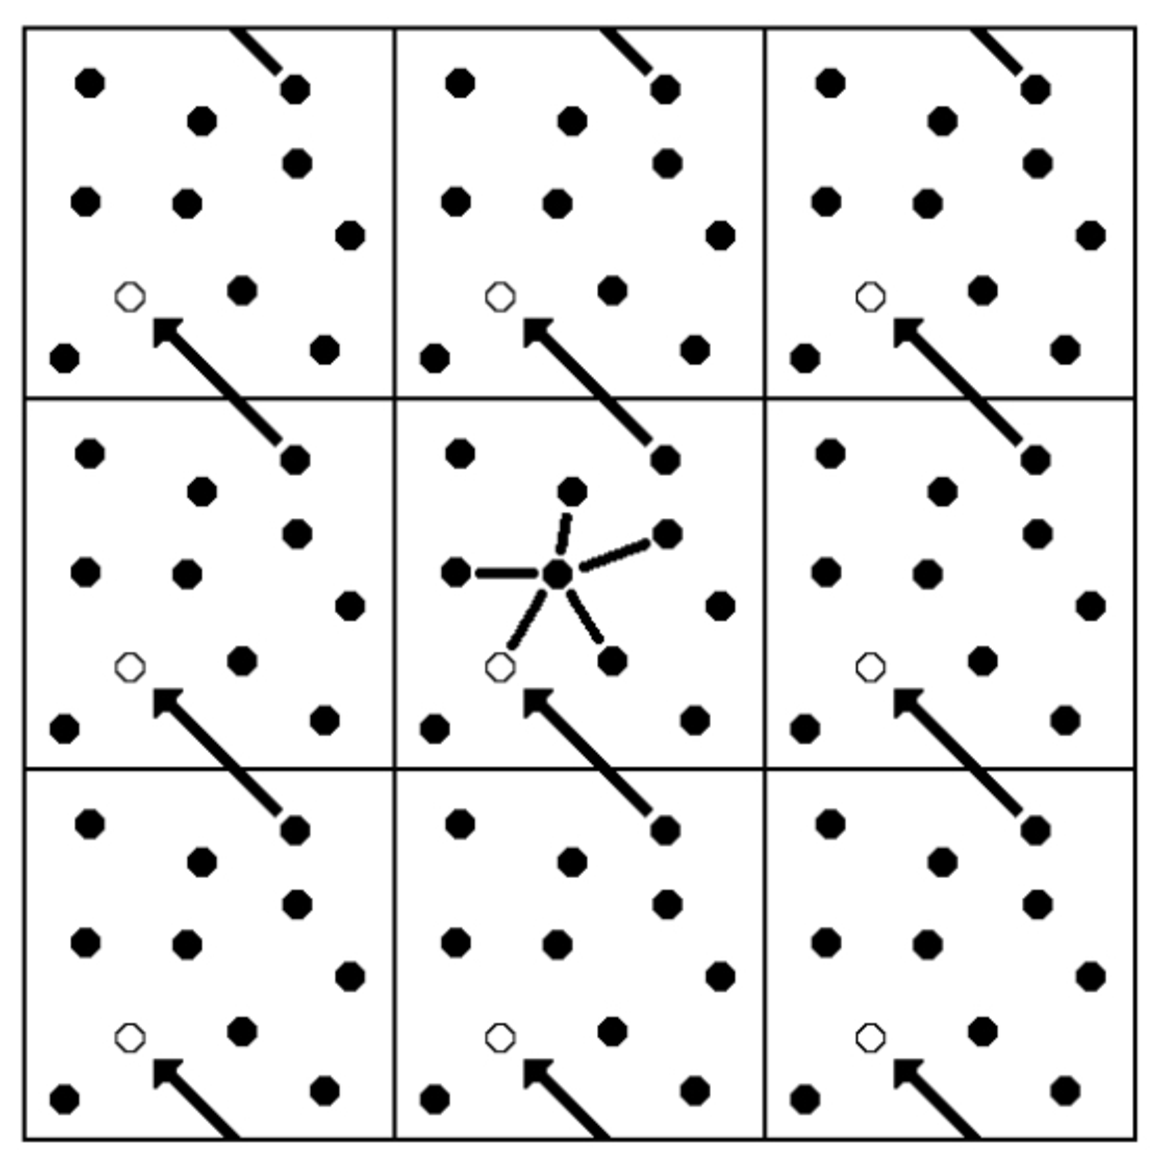
\includegraphics[scale=0.3]{contorno}
\end{center}
\caption{\label{condcont} {\sl Condições periódicas de contorno na simulação.}}
\end{figure}

Este 
processo esta
esquematizado na Figura \ref{condcont}.
Para verificar se uma partícula conseguiu sair da caixa de simulação e 
consequentemente outra
entrou, usamos condições de contorno periódicas. Para
exemplificar isto consideremos que após um deslocamento a partícula ocupa
a posição ($x,y,z$). Para verificar se a coordenada $x$ ($y,z$) da partícula
encontra-se dentro ou fora da caixa utilizamos a função definida como

\begin{equation} \label{b1}
x=x+\frac{L_x}{2} \; {\rm anint}(-2x/L_x)
\end{equation}

\noindent onde $L_x$ representa o comprimento do lado $x$ da caixa de
simulação, anint é uma função da forma

\begin{equation}
{\rm anint} = \left\{\begin{array}{l}
    \hspace{0.3cm}  1, \; \; {\rm se} \; \; \;  -2x/L_x > 1  \\
    \hspace{0.3cm}  0, \; \; {\rm se} \; \; \; -1 \le -2x/L_x \le 1 \\
             -1, \; \; {\rm se} \; \; \; -2x/L_x < 1
                     \end{array} \right.
\end{equation}

\newpage

\chapter{Parâmetros dos potenciais usados} \label{potparam}

Alguns parâmetros são apresentados com um número de casas maior que o número
significativo para
garantir precisão computacional.

\section{HFD-B3-FCI1 - $V_h$}

\begin{equation} \nonumber
\begin{array}{ccc}
\epsilon=10.9560000 \; {\rm K}, & & C_6=1.35186623, \\
r_m=2.9683000 \; {\rm \mathring{A}}, & & C_8=0.41495143,\\
D=1.43800000, & & C_{10}=0.17151143, \\
\alpha=10.5717543, & & A=1.86924404 \times 10^5, \\
\beta=-2.07758779.
\end{array}
\end{equation}

\section{Korona e colaboradores - $V_p$}

\begin{equation} \nonumber
\begin{array}{ccccc}
C_6=1.4609778 \; {\rm (a.u)}, & & C_8=14.117855 \; {\rm (a.u)} ,& & 
C_{10}=183.69125 \; {\rm
(a.u)}, \\
C_{12}=3265 \; {\rm (a.u)}, & & C_{14}=76440 \; {\rm (a.u)}, & & 
C_{16}=2275000 \; {\rm (a.u)},
\\
A=2074364.26 \; {\rm K}, & & \alpha=1.88648251 \; {\rm bohr}^{-1}, & & 
\beta=-0.062001349 \;
{\rm
bohr}^{-2}, \\
b=1.94861295 \; {\rm bohr}^{-1}.
\end{array}
\end{equation}

\section{Janzen e colaboradores - $V_{pr}$}

Os valores dos parâmetros para este potencial são os mesmos que para o 
potencial $V_p$. A função
de retardo $f_r(r)$ esta definida como


\begin{table}[h]
\centering
{\small
\begin{tabular}{|ccc|}
\hline \hline
{\rm Intervalo $r$} & $f_r(r)$ & $p_1$ (a.u.) \\
\hline \hline
$0 \le r <5.7$ & 1 & ----- \\
$5.7 \le r <10$ & $p_1+p_2r+p_3r^2+p_4r^3$ & $9.860029\times10^{-1}$ \\
$10 \le r <10^2$ & $1-p_1-p_2r^{0.5}-p_3r-p_4r^{1.5}-p_5r^2$ & 
$-1.62343\times10^{-3}$ \\
$10^2 \le r <2\times10^2$ & $(1+p_1+p_2r^{0.5}+p_3r+p_4r^2)/(1.2+0.8p_5r)$ &
$8.82506\times10^{-2}$ \\
$2\times10^2 \le r <10^3$ & ${\rm ln}(r(p_1r^{0.4}+p_2r^{0.5}+p_3r^{0.6}
+p_4r^{0.7}+p_5r^{0.8}))$ & $1.488897$ \\
$10^3 \le r <10^4$ & $p_1+p_2/r+p_3/r^2+p_4/r^3+p_5/r^4$ & 
$6.184108\times10^{-6}$ \\
$10^4 \le r <10^5$ & $p_1+p_2/r+p_3/r^2+p_4/r^3+p_5/r^4$ & 
$-1.107002\times10^{-7}$ \\
\hline \hline
\end{tabular}}
\end{table}

\begin{table}[h]
\centering
{\small
\begin{tabular}{|ccccc|}
\hline \hline
{\rm Intervalo $r$} & $p_2$ (a.u.)& $p_3$ (a.u.)& $p_4$ (a.u.)& $p_5$ 
(a.u.)\\
\hline \hline
0 $\le$ r <5.7 & ----- & ----- & ----- & ----- \\
5.7 $\le$ r <10 & $5.942027\times10^{-3}$ & $-7.924833\times10^{-4}$ & 
$3.172548\times10^{-5}$ &
----- \\
10 $\le$ r <$10^2$ & $2.22097\times10^{-3}$ & $-1.17323\times10^{-3}$ & 
$3.00012\times10^{-4}$ &
$-1.05512\times10^{-5}$ \\
$10^2$ $\le$ r <$2\times10^2$ & $3.81846\times10^{-2}$ & 
$-1.72421\times10^{-3}$ &
$4.74897\times10^{-7}$ & $3.0445706\times10^{-3}$ \\
$2\times10^2$ $\le$ r <$10^3$ & $-2.123572$ & $1.043994$ & 
$-1.898459\times10^{-1}$ &
$6.479867\times10^{-3}$ \\
$10^3$ $\le$ r <$10^4$ & $3.283043\times10^2$ & $1.367922\times10^3$ & 
$-4.464489\times10^7$ &
$1.365003\times10^{10}$ \\
$10^4$ $\le$ r <$10^5$ & $3.284717\times10^2$ & $-9.819846\times10^2$ & 
$-1.953816\times10^7$ &
$-1.079712\times10^{11}$ \\
\hline \hline
\end{tabular}}
\end{table}

\section{HFDHE2 - $V_A$}

\begin{equation} \nonumber
\begin{array}{ccc}
\epsilon=10.8 \; {\rm K}, & & C_6=1.3732412, \\
r_m=2.9673 \; {\rm \mathring{A}}, & & C_8=0.4253785,\\
D=1.241314, & & C_{10}=0.178100, \\
\alpha=13.353384, & & A=0.5448504 \times 10^6.
\end{array}
\end{equation}

\section{Cohen e Murrell - $V_3$}

\begin{equation} \nonumber
\begin{array}{ccccc}
k=2.7 \; {\rm \mathring{A}}, & & \alpha=3.446 \; {\rm \mathring{A}^{-1}}, & 
& l=1.15, \\
c_0=-1957.895, & & c_1=673.186, & & c_2=-188.491, \\
c_3=3664.836, & & c_4=-1655.476, & & c_5=244.090, \\
c_6=4129.947, & & c_7=-1726.015, & & c_8=177.661, \\
c_9=2693.277, & & c_{10}=-1096.591, & & c_{11}=154.063, \\
c_{12}=6011.520, & & c_{13}=-2618.297, & & c_{14}=296.384 \;.
\end{array}
\end{equation}

\noindent Os parâmetros $c_i$ estão nas unidades apropriadas, {\sl i.e.}, $c_0=eV_h$, 
$c_1=eV_h/{\rm \mathring{A}}$, etc.

\noindent Aqui $1eV_h=0.036726 E_h$.

\end{document}


